\documentclass{standalone}
\usepackage{tikz}
\usetikzlibrary{positioning}

% To convert the document to a png:
% magick convert -density 200  -trim filename.pdf -quality 100 filename.png


\begin{document}
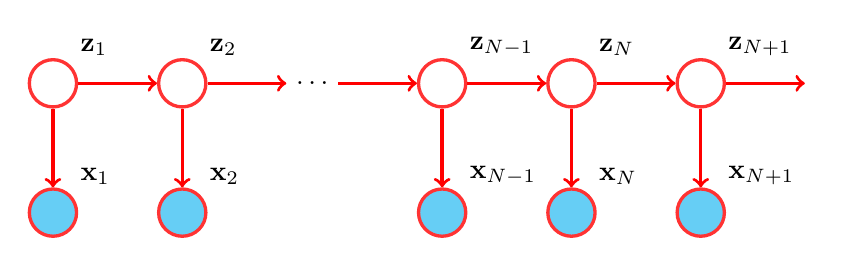
\begin{tikzpicture}[
latentnode/.style={circle, draw=red!80, minimum size=6mm, very thick},
observednode/.style={circle, draw=red!80, fill=cyan!60, minimum size=6mm, very thick},
]

% Defining the nodes
\node[latentnode, label=above right:{${\bf z}_1$}] (z1) {};
\node[latentnode, label=above right:{${\bf z}_2$}] (z2) [right=of z1] {};
\node (transition) [right=of z2] {$\ldots$};
\node[latentnode, label=above right:{${\bf z}_{N-1}$}] (z_nm1) [right=of transition] {};
\node[latentnode, label=above right:{${\bf z}_{N}$}] (zn) [right=of z_nm1] {};
\node[latentnode, label=above right:{${\bf z}_{N+1}$}] (z_np1) [right=of zn] {};
\node (final) [right=of z_np1] {};

% Defining observed nodes
\node[observednode, label=above right:{${\bf x}_1$}] (x1) [below=of z1]{};
\node[observednode, label=above right:{${\bf x}_2$}] (x2) [below=of z2]{};
\node[observednode, label=above right:{${\bf x}_{N-1}$}] (x_nm1) [below=of z_nm1]{};
\node[observednode, label=above right:{${\bf x}_{N}$}] (xn) [below=of zn]{};
\node[observednode, label=above right:{${\bf x}_{N+1}$}] (x_np1) [below=of z_np1]{};


% Relationships between latent variables
\draw[->, color=red, very thick] (z1) -- (z2);
\draw[->, color=red, very thick] (z2) -- (transition);
\draw[->, color=red, very thick] (transition) -- (z_nm1);
\draw[->, color=red, very thick] (z_nm1) -- (zn);
\draw[->, color=red, very thick] (zn) -- (z_np1);
% final node
\draw[->, color=red, very thick] (z_np1) -- (final);

% Relationships between observed and latent variables
\draw[->, color=red, very thick] (z1) -- (x1);
\draw[->, color=red, very thick] (z2) -- (x2);
\draw[->, color=red, very thick] (z_nm1) -- (x_nm1);
\draw[->, color=red, very thick] (zn) -- (xn);
\draw[->, color=red, very thick] (z_np1) -- (x_np1);

\end{tikzpicture}

\end{document}
